\documentclass{article}
\usepackage{import}
\usepackage{amsmath}
\usepackage{tabularray}
\usepackage{float}
\import{lib/latex/}{wgmlgz}
\patchcmd{\thebibliography}{\section*}{\section}{}{}

\begin{document}
\itmo[
      variant=13,
      labn=1,
      discipline=Вычислительная математика,
      group=P3212,
      student=Соколов Анатолий Владимирович,
      teacher=Наумова Надежда Александровна 
]
\lstset{language=rust}
\newgeometry{
  a4paper,
  top=20mm,
  right=10mm,
  bottom=20mm,
  left=30mm
}
\tableofcontents

\section{Задание}
% \begin{enumerate}

В программе реализуемый численный метод решения системы линейных алгебраических уравнений (СЛАУ) должен быть реализован в виде отдельного класса /метода/функции, в который исходные/выходные данные передаются в качестве параметров.
\\
Задавать размерность матрицы ($n<20$) из файла или с клавиатуры ‒ по выбору конечного пользователя.
\\      
Должна быть реализована возможность ввода коэффициентов матрицы, как с клавиатуры, так и из файла (по выбору конечного пользователя).
\\
Сформировать не менее 3 файлов (тестов) с различным набором данных.
\\
Программа должна быть протестирована на различных наборах данных, в том числе и некорректных.

\subsection{Вариант}

\bold{Для итерационных методов должно быть реализовано:}

\begin{center}
      % \includegraphics[width=175pt]{opd/4/4.png}
      \begin{itemize}
      \item Точность задается с клавиатуры/файла
      \item Проверка диагонального преобладания (в случае, если диагональное преобладание в исходной матрице отсутствует, сделать перестановку строк/столбцов до тех пор, пока преобладание не будет достигнуто). В случае невозможности достижения диагонального преобладания - выводить соответствующее сообщение.
      \item Вывод вектора неизвестных: $x1$, $x2$, $\dots$ , $xn$
      \item Вывод количества итераций, за которое было найдено решение.
      \item Вывод вектора погрешностей: $|x_i^K-x_i^{k-1}|$
      \end{itemize}
      \end{center}

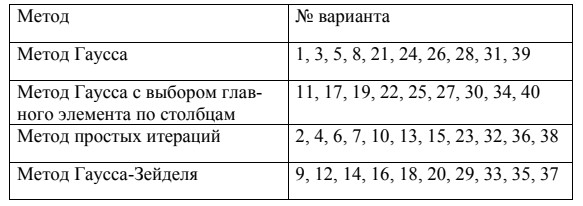
\includegraphics{task.jpg}

\begin{lstlisting}
fn shuffle(&mut self) -> (bool, Vec<Vec<f64>>) {
      let mut biggest = vec![-1; self.n];
      let mut biggest_set = HashSet::new();
      let mut found_strict = false;

      for i in 0..self.n {
            let sum: f64 = self.a[i].iter().sum();
            for j in 0..self.n {
                  if 2.0 * self.a[i][j] >= sum {
                  if 2.0 * self.a[i][j] > sum {
                        found_strict = true;
                  }
                  biggest[i] = j as isize;
                  biggest_set.insert(j);
                  break;
                  }
            }
            if biggest[i] == -1 {
                  return (false, vec![vec![0.0]]);
            }
      }

      if !found_strict || biggest.len() != biggest_set.len() {
            return (false, vec![vec![0.0]]);
      }

      let mut shuffled_a = vec![vec![]; self.n];
      let mut shuffled_b = vec![0.0; self.n];

      for i in 0..self.n {
            let index = biggest[i] as usize;
            shuffled_a[index] = self.a[i].clone();
            shuffled_b[index] = self.b[i];
      }

      self.a = shuffled_a.clone();
      self.b = shuffled_b;

      (true, shuffled_a)
      }

fn find_c_and_d(coefficients: Vec<Vec<f64>>) -> Vec<Vec<f64>> {
      let n = coefficients.len(); // The number of rows, assuming a square matrix for coefficients
      let mut c = vec![vec![0.0; n]; n]; // Initialize C matrix with zeros

      for i in 0..n {
            // Diagonal element of the current row
            let diag_elem = coefficients[i][i];

            for j in 0..n {
                  // Check if the current element is not on the diagonal
                  if i != j {
                  // C matrix is -1 times the original coefficient matrix divided by the diagonal element
                  c[i][j] = -coefficients[i][j] / diag_elem;
                  }
            }
            // The diagonal elements of C are set to zero
            c[i][i] = 0.0;
      }

      c
      }

fn iterate(&mut self) {
      let mut new_sol = vec![0.0; self.n];
      for i in 0..self.n {
            new_sol[i] = self.b[i] / self.a[i][i] - self.sum_sol_row(i);
            self.sol_acc[i] = (new_sol[i] - self.sol[i]).abs();
      }
      self.sol = new_sol;
      self.sol_iter += 1;
      }

      pub fn solve(&mut self) -> Json<serde_json::Value> {
      let mut err = String::new();

      if !self.shuffle().0 {
            err = String::from("Невозможно привести к диагональному преобладанию.")
      }

      self.shuffled_matrix = self.shuffle().1;

      while self.sol_acc.iter().max_by(|a, b| a.total_cmp(b)).unwrap() > &self.acc
            && self.sol_iter < self.max_iter
      {
            self.iterate();
      }
      // self.print_sol();

      if !self.shuffled_matrix.is_empty() {
            self.c = Matrix::find_c_and_d(self.shuffle().1);
            return Json(json!({
                  "sol": self.sol,
                  "acc": self.sol_acc,
                  "iter": self.sol_iter,
                  "c": self.c,
                  "mtrx": self.shuffled_matrix,
                  "err": err,
            }));
      }

      Json(json!({
            "sol": self.sol,
            "acc": self.sol_acc,
            "iter": self.sol_iter,
            "mtrx": self.shuffled_matrix,
            "err": err,
      }))
      }
\end{lstlisting}

\section{Заключение}
Я познакомился с новым для меня и крайне необыкновенным функционалом работы серверной системы с названием «Гелиос», ознакомился со стеком html, css, js, php. Прекраснейше провел время, программируя на языке PHP, обладающим великолепным синтаксисом.

\begin{thebibliography}{9}
    \bibitem{Методичка}Слайды с лекций (2023). // Кафедра информатики и вычислительной техники -- Малышева Татьяна Алексеевна, к.т.н., доцент.
\end{thebibliography} 

\end{document}
